\documentclass[twocolumn]{jsarticle}

\usepackage{amsmath,amsfonts}
\usepackage{bm}
\usepackage[dvipdfmx]{graphicx}
\usepackage[dvipdfmx]{hyperref}
\hypersetup{
  setpagesize=false,
  bookmarksnumbered=true,
  bookmarksopen=true,
  colorlinks=true,
  linkcolor=blue,
  citecolor=red
}
\usepackage{url}
\usepackage{ascmac}
\usepackage{caption}


\renewcommand{\thefigure}{\arabic{figure}}
\begin{document}


\title{\vspace{-3cm}大規模言語モデルの性能評価を目的とした\\
文脈情報に基づく日本語テストデータの自動生成}
\author{
  システム情報工学研究群 情報理工学位プログラム\\
  前期博士課程2年 202420612 佐多 亮明\\
  指導教員: 山本 幹雄
}
\date{2025年7月5日}
\maketitle



\section{背景}
近年、大規模言語モデル(LLM)は急速な発展を遂げており、その応用範囲は多岐にわたる。この技術の健全な発展のためには、各モデルの能力を正確に理解し、比較するための信頼性の高い評価手法が不可欠である。しかし、特に日本語ドメインにおいては、モデルの性能を多角的に測定するための高品質な評価データセット(ベンチマーク)が不足しているという課題が存在する。

従来、こうした評価データセットは人手によるアノテーションを通じて作成されてきた。このアプローチは品質を担保する上でのゴールドスタンダードであるが、膨大な時間と金銭的コストを要するという大きな制約を抱えている。結果として、次々と登場する新しいモデルの開発スピードに、評価データセットの整備が追いつかないという事態が生じている。

このコストと時間の問題を解決する有望な代替案として、LLM自体に評価データを自動生成させるアプローチが考えられる。しかし、この手法には「ハルシネーション(幻覚)」という重大な課題がつきまとう。事実に基づかない情報を生成してしまうLLMの性質上、信頼できる情報源なしにデータを生成させると、内容が不正確であったり、問題として成立していなかったりする質の低いデータが大量に作られてしまう。

そこで本研究では、ハルシネーションを抑制し、事実に基づいた高品質なテストデータを自動生成する手法を提案する。具体的には、Wikipedia記事のような信頼できる「文脈(コンテキスト)」をLLMに与え、そのテキスト内容に完全に準拠した一問一答形式のテストデータを生成させる。本研究の目的は、この手法で生成したテストデータセットが、人手で作成された既存のベンチマークと同様に、様々なLLMの性能序列を正確に反映できるかを実証することにある。これにより、低コストかつ大規模な評価データセットの持続的な供給を可能にし、日本語LLMの研究開発エコシステムの発展に貢献することを目指す。



\section{関連研究}

\subsection{JSQuAD}
JSQuADは、Yasunagaらによって構築された\cite{JSQuAD}、日本語の読解能力を評価するための大規模なデータセットである。これは、機械読解の分野で広く標準的なベンチマークとして利用されている英語のSQuAD\cite{SQuAD}の日本語版にあたる。データセットの構築は、日本語版Wikipediaの記事を文脈情報とし、クラウドソーシングを通じて作業者が文脈に関する「質問」と、その「回答」となる箇所を文脈中から抜き出す(スパン形式)ことで行われた。

このデータセットは、日本語を扱う言語モデルの読解能力と質問応答能力の向上に向けた学習および性能評価基盤を提供することを目的としている。本研究では、このJSQuADを2つの重要な役割で活用する。第一に、提案手法である指示チューニングにおいて、その高品質な「文脈・質問・回答」の三つ組を、QAペア生成モデルの学習用教師データとして用いる。第二に、自動生成されたテストデータセットの有効性を評価する上で、JSQuADを人間が作成した基準として利用し、各LLMの性能ランキングを比較するためのベンチマークとする。

% fig ディレクトリから画像を挿入
\begin{figure*}[t]
  \centering
  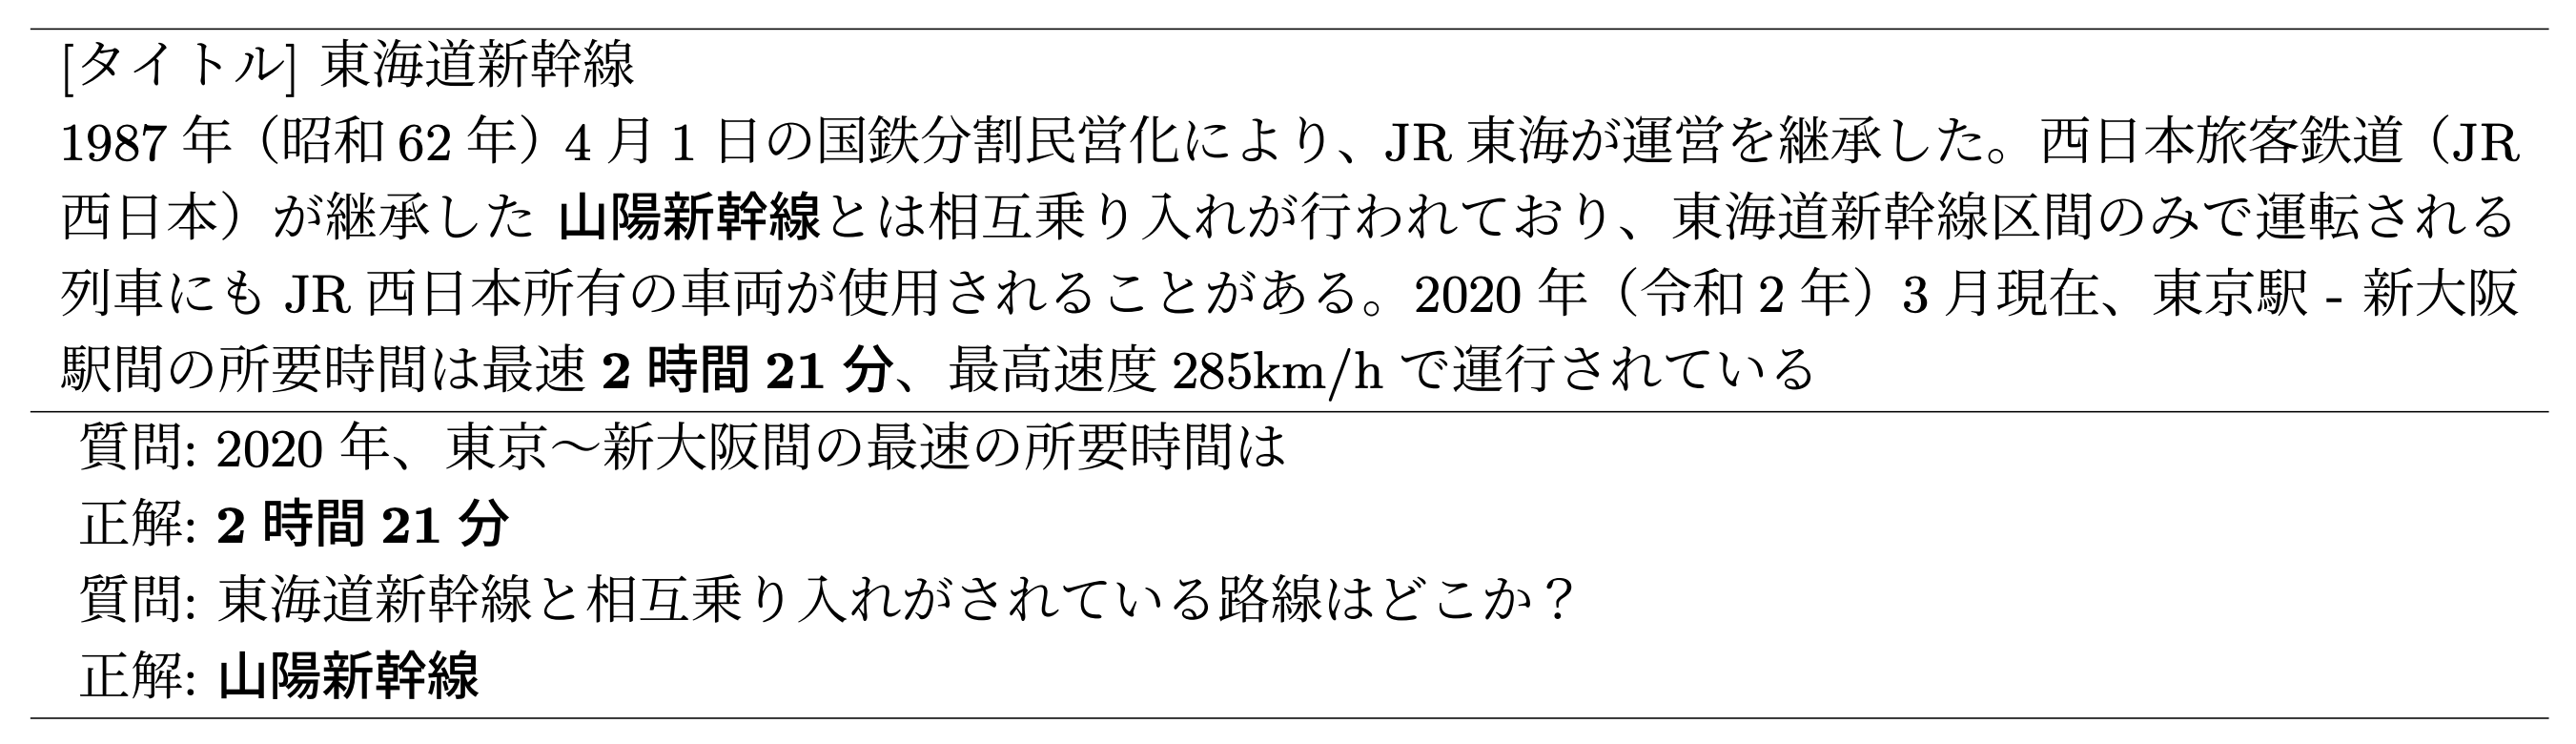
\includegraphics[width=\linewidth]{fig/jsquad.png}
  \caption{JSQuADのデータ構造例}
  \label{fig:jsquad_example}
\end{figure*}

\subsection{指示チューニング}
指示チューニングは、Weiらによって提案された\cite{Instruction-Tuning}、事前学習済みのLLMを、多様なタスクを記述した指示(instruction)の集合で微調整(ファインチューニング)する手法である。その目的は、モデルが未学習のタスクに対しても、タスク内容を説明した指示を理解するだけでゼロショットで対応できる汎化能力を獲得させることにある。

この手法のプロセスでは、翻訳、要約、質問応答といった様々な既存のNLPタスクを、「この文章を要約してください」のような自然言語の指示テンプレートを用いて表現し、それらを大規模に組み合わせたデータセットでモデルを微調整する。この研究により、単一のタスクでファインチューニングするのではなく、多種多様なタスクを統一的な指示形式で学習させることが、LLMの汎化性能を劇的に向上させることが示された。また、その効果は「モデルの規模(スケール)」と「チューニングに用いるタスクの数と多様性」が豊かであるほど高まることも明らかにされており、後の多くのLLM開発における基本方針となっている。

\subsection{指示事前学習 (Instruction Pre-Training)}
指示事前学習は、Chengらによって提案された\cite{Instruction Pre-Training}、言語モデルの事前学習段階そのものに指示データを組み込む新しいフレームワークである。従来の手法と異なり、生コーパスとその内容に基づき自動生成した「指示と応答」のペアを組み合わせた「指示拡張コーパス」を用いて事前学習を行う。このアプローチの目的は、従来ファインチューニング段階で行われてきた教師ありマルチタスク学習の利点を、モデルの基礎能力を形成する事前学習段階に取り込むことにある。

この手法で用いられる指示生成の着想は、本研究における「JSQuADのデータ構造を組み替えて指示チューニングデータを作成する」というアプローチと共通点が多い。しかし、本論文がモデルの汎用的な能力向上を目指して事前学習の段階で指示データを導入するのに対し、本研究では評価用データセットの生成という特定の目的のためにファインチューニング段階で指示チューニングを活用する点で、目的と適用段階が明確に異なる。



\section{提案手法}

本研究では、信頼性の高い日本語テストデータを自動生成する手法を提案し、その有効性を検証する。具体的には、生成モデルとして日本語処理能力に優れたtokyotech-llm/Llama-3.1-Swallow-8B-Instruct-v0.3\cite{Fujii:COLM2024}\cite{Okazaki:COLM2024}\cite{ma:arxiv2025}を用い、与えられた文脈情報から一問一答形式のQAペアを生成させる。その生成アプローチとして、本研究の主軸となる「指示チューニング」\cite{Instruction-Tuning}に加えて、比較対象となる「Zero-Shot推論」や「Few-Shot推論」を実装する。

前述の指示チューニングでは、人間が作成した高品質な読解データセットであるJSQuAD\cite{JSQuAD}を学習用途として効果的に活用し、高品質なテストデータを自動生成する。本来、JSQuADは「文脈」と「質問」が与えられた際に「回答」を予測する読解タスク用に設計されている。本研究ではこの入出力構造を意図的に組み替え、「文脈」のみを入力として、対応する「質問と回答のペア」全体を出力するようにタスクを再定義した。この発想の転換により、読解モデル評価用のデータセットを、QAペア生成モデルの学習用教師データとして活用することが可能となる。これにより、モデルは文脈から適切な問いと答えを創出する能力を直接的に学習し、学習後にはプロンプトと未知の文脈を入力するだけで、その内容に基づいたQA形式のテストデータを生成できるようになる。

また、指示チューニングの有効性を示すために、Zero-Shot推論とFew-Shot推論の2つのアプローチも比較対象として実装する。Zero-Shot推論では、プロンプトに「この文章に基づいて質問と回答を生成してください」といった一般的な指示を与える。一方、Few-Shot推論では、JSQuADのデータセットから抽出したいくつかのQAペアをプロンプトに含め、モデルがそのパターンを学習できるようにする。

上記のアプローチで生成した各テストデータセットの有効性を評価するため、統一された評価フレームワークを構築した。性能評価の基準(ベースライン)として、人間が作成したJSQuADデータセットを本来の読解タスクとして用いる。この基準データセットを12種類のオープンソースLLM群に解かせ、それぞれの正解率(回答の完全一致率)を基に「モデル性能の基準ランキング」を算出する。次に、自動生成した各テストデータセットを用いて同様に12モデルの性能ランキングをそれぞれ算出する。最終的に、「基準ランキング」と「自動生成データによるランキング」との間にどの程度の相関があるかを、スピアマンの順位相関係数($\rho$)を用いて定量的に評価する。この$\rho$値が1に近いほど、自動生成されたテストデータが、人手によるベンチマークと同等の信頼性を持つ評価軸として機能することを示す。



\section{実験と考察}

提案手法の有効性を実証するため、自動生成されたテストデータセットを用いてLLMの性能評価実験を行った。実験設定は3章で述べた通りである。本実験の目的は、各自動生成アプローチが、JSQuAD\cite{JSQuAD}を基準として算出されたベースラインランキングをどの程度忠実に再現できるかを定量的に示すことにある。

各生成アプローチ(Zero-Shot, Few-Shot, 指示チューニング)で作成したテストデータセットと、ベースラインランキングとのスピアマンの順位相関係数($\rho$)を表\ref{tab:rho_summary}にまとめる。

\begin{table}[h]
  \centering
  \caption{各生成アプローチと順位相関係数の比較}
  \label{tab:rho_summary}
  \begin{tabular}{lc}
  \hline
  生成アプローチ       & 順位相関係数 ($\rho$) \\
  \hline
  Zero-Shot 推論       & 0.6364                     \\
  10-Shot 推論         & 0.7622                     \\
  指示チューニング(提案手法) & 0.8741                     \\
  \hline
  \end{tabular}
\end{table}

表\ref{tab:rho_summary}が示す通り、相関係数はZero-Shot推論の$\rho=0.6364$から、Few-Shot推論で$\rho=0.7622$へ、そして指示チューニングでは$\rho=0.8741$へと段階的に向上した。この傾向は、生成モデルへの指示をより具体的に、かつタスクに特化させるほど、生成されるテストデータセットの信頼性が向上することを示唆している。

特に、本研究の主軸である指示チューニングアプローチが高い相関を達成したことは、JSQuADのデータ構造を組み替えて学習させるという本手法の有効性を強く裏付けている。これにより、人間が作成したベンチマークの評価軸を極めて忠実に再現可能であることが実証された。なお、自動生成データを用いた際の各モデルの絶対的な正解率は、人間製データで評価した際よりも全体的に低下する傾向が見られた。これは生成された問題の難易度や表現の揺れに起因すると考えられる。しかし、評価データセットとしての最も重要な役割である、モデル間の相対的な性能差を正確に捉え、信頼性の高い性能ランキングを構築するという点において、本提案手法は十分に有効であることが、この高い順位相関係数によって示されている。



\section{今後の展望}

本研究では、文脈情報に基づく一問一答形式のテストデータを自動生成し、その有効性を示した。この成果を基盤とし、将来的には以下のような方向性で研究を発展させることを目指す。

第一に、生成データの品質を強化学習によってさらに向上させることである。本稿で示した指示チューニングは高い有効性を示したが、生成される回答の形式をより厳密に制御するには限界がある。そこで、指示チューニング済みモデルに対し、GRPOなどの強化学習手法を適用するアプローチが考えられる\cite{Instruction Pre-Training}。例えば、「回答が文脈から抽出可能であること」「回答が簡潔な名詞句であること」「質問と文脈の関連性が高いこと」といった理想的なテストデータが満たすべき条件を報酬関数として設計し、モデルを最適化する。これにより、評価の安定性をさらに高めることができると期待される。

第二に、異言語データセットを活用した生成モデルの構築である。本研究は日本語のJSQuAD\cite{JSQuAD}を基盤としたが、高品質な学習データが存在しない言語や専門ドメインも多い。この課題に対し、英語圏の豊富なデータセット(例:SQuAD\cite{SQuAD})で指示チューニングを行ったモデルを、日本語のテストデータ生成に応用する研究が有望である。単純な適用では言語の壁があるため、英語で得た汎用的なQA生成能力を、少量の日本語データで効率的に適応させる技術などを探求することで、多言語・多ドメインへの応用可能性が拓ける。

最後に、より高度な推論能力を測定するためのテストフォーマットへの拡張である。現在の抽出型QA形式に加え、より複雑な能力を評価できるデータセットの生成を目指す。具体的には、正解以外の魅力的な誤答選択肢を自動生成する「複数選択肢形式」や、文脈中の複数箇所に散らばった情報を統合して初めて解答可能となる「マルチホップ質問応答」への対応を検討する。これらの実現は、LLMの評価を単なる知識の検索から、より深い論理的推論能力の測定へと進化させると考えられる。



\begin{thebibliography}{99}
  \bibitem{Instruction-Tuning}
  Jason Wei, Maarten Bosma, Vincent Y. Zhao, Kelvin Guu, Adams Wei Yu, Brian Lester, Nan Du, Andrew M. Dai, Quoc V. Le. Finetuned Language Models Are Zero-Shot Learners. arXiv:2109.01652. 2021.
  \bibitem{Instruction Pre-Training}
  Daixuan Cheng, Yuxian Gu, Shaohan Huang, Junyu Bi, Minlie Huang, Furu Wei. Instruction Pre-Training: Language Models are Supervised Multitask Learners. arXiv:2406.14491. 2024.
  \bibitem{SQuAD}
  Pranav Rajpurkar, Jian Zhang, Konstantin Lopyrev, Percy Liang. SQuAD: 100,000+ Questions for Machine Comprehension of Text. arXiv:1606.05250. 2016.
  \bibitem{JSQuAD}
  Soichi Yasunaga, Juro Fukunaga, et al. JSQuAD: A Japanese Question Answering Dataset. arXiv:2202.01764. 2022.
  \bibitem{JGLUE}
  Kurihara Kentaro, Kawahara Daisuke, Shibata Tomohide. JGLUE: Japanese General Language Understanding Evaluation. https://aclanthology.org/2022.lrec-1.317. 2022.
  \bibitem{Fujii:COLM2024}
  Kazuki Fujii, Taishi Nakamura, Mengsay Loem, Hiroki Iida, Masanari Ohi, Kakeru Hattori, Hirai Shota, Sakae Mizuki, Rio Yokota, Naoaki Okazaki. Continual Pre-Training for Cross-Lingual LLM Adaptation: Enhancing Japanese Language Capabilities. Proceedings of the First Conference on Language Modeling. 2024.
  \bibitem{Okazaki:COLM2024}
  Naoaki Okazaki, Kakeru Hattori, Hirai Shota, Hiroki Iida, Masanari Ohi, Kazuki Fujii, Taishi Nakamura, Mengsay Loem, Rio Yokota, Sakae Mizuki. Building a Large Japanese Web Corpus for Large Language Models. Proceedings of the First Conference on Language Modeling. 2024.
  \bibitem{ma:arxiv2025}
  Youmi Ma, Sakae Mizuki, Kazuki Fujii, Taishi Nakamura, Masanari Ohi, Hinari Shimada, Taihei Shiotani, Koshiro Saito, Koki Maeda, Kakeru Hattori, Takumi Okamoto, Shigeki Ishida, Rio Yokota, Hiroya Takamura, Naoaki Okazaki. Building Instruction-Tuning Datasets from Human-Written Instructions with Open-Weight Large Language Models. arXiv:2503.23714. 2025.
\end{thebibliography}

\end{document}
